
\chapter{Least squares and maximum likelihood}
\section{The mean}\label{sec:mean}
\subsection{Least squares}
These notes are for regression. So now is the time to know that regression produces a conditional mean (a mean that exists under certain specified conditions). Since learning regression is what we are here to do, it makes sense to show how useful means really are. If we use as our criteria for whether a summary statistic about the data is "good" or not is the deviation between the observation and our statistic, then we want a summary statistic to minimize these differences.

As mentioned earlier, adding up all of the deviances will produce 0. To circumvent this problem, the deviances were squared and then added up. Therefore, we want our mystery statistic, $\theta$ to be a {\it function} of these squared deviations:
\begin{equation}
S\left(\theta\right)=\sum_{i=1}^{N}e_i^2=\sum_{i=1}^{N}\left(x_i-\theta\right)^2
\end{equation}
A "good" estimate will have the least amount of differences. Thus, we want our statistic to minimize $\sum_{i=1}^{N}\left(x_i-\theta\right)^2$. So, how to we figure out which statistics will minimize the sum of these squared deviations? Let's break it down into known and unknown quantities. Someone smarter than me figured out that if you rearrange the terms, you can express this function as
\[
S\left(\theta\right)=\sum_{i=1}^{N}\left(x_i-\theta\right)^2
\]
factor it
\[
S\left(\theta\right)=\sum_{i=1}^{N}\left(\left(x_i-\theta\right)\left(x_i-\theta\right)\right)
\]
\[
S\left(\theta\right)=\sum_{i=1}^{N}\left(x_i^2-x_i\theta-x_i\theta+\theta^2\right)
\]
\[
S\left(\theta\right)=\sum_{i=1}^{N}\left(x_i^2-2x_i\theta+\theta^2\right)
\]
then take the elements out of the summation
\begin{equation}
S\left(\theta\right)=\sum_{i=1}^{N}x_i^2-2\theta\sum_{i=1}^Nx_i+N\theta^2
\end{equation}
Since, theoretically, we know our data, and thus know the sum of x squared, $\sum_{i=1}^{N}x_i^2$ , and the sum of x, $\sum_{i=1}^{N}x_i$, and $N$, then this function only has one unknown, $\theta$. We can use calculus to find the first derivative of this function with respect to $\theta$. Relying on the fact that the derivative of a sum of functions is the sum of the derivatives of each function, we can find the derivative of each element. The derivative of $\sum_{i=1}^{N}x_i^2$ is 0, since it is a constant and doesn't involve $\theta$, the derivative of $-2\theta\sum_{i=1}^Nx_i$ with respect to $\theta$ is $-2\sum_{i=1}^Nx_i$, and finally the power rule tells us that the derivative of $N\theta^2$ is $2N\theta$. Adding this all together gets us the derivative of the function with respect to $\theta$ as
\begin{equation}
\frac{dS\left(\theta\right)}{d\left(\theta\right)}=-2\sum_{i=1}^{N}x_i+2N\theta
\end{equation}
Then we set this first derivative to 0 (the first derivative of a function is its slope, and when the slope of a function is zero, the function is at a minimum or maximum) and solve for $\theta$:
\[
0=-2\sum_{i=1}^{N}x_i+2N\theta
\]
\[
2\sum_{i=1}^{N}x_i=2N\theta
\]
\[
\sum_{i=1}^{N}x_i=N\theta
\]
\[
\frac{\sum_{i=1}^{N}x_i}{N}=\theta
\]
Now that we have it, we name the statistic $\mu$ and also call it the mean, c.f.~\eqref{eq:mean}. For example, Table~\ref{tab:desx} presents some random numbers and the key statistics to graph the least squares function. For Table~\ref{tab:desx} this function is
\[
S\left(\theta\right)=\sum_{i=1}^{N}x_i^2-2\theta\sum_{i=1}^{N}x_i+N\theta^2
\]
\[
S\left(\theta\right)=9887.521-2\theta 988.596+N\theta^2
\]
and this function is visualized in Figure~\ref{fig:sse}. I show that the mean we estimate does indeed present the minimum sum of squared errors. Any other value for the mean increases error.

\begin{table}[htbp]\centering
\caption{Random variable $x$\label{tab:desx}
\textbf{} }\begin{tabular} {@{} ccccc @{}} \\
\hline
10.939&10.470&10.333&8.738&9.827 \\
10.279&9.754&10.261&11.036&10.054 \\
10.637&10.659&10.742&10.492&11.260 \\
10.378&9.007&10.092&9.430&10.618 \\
8.147&10.414&10.250&9.378&9.728 \\
10.338&8.780&10.539&10.504&8.474 \\
8.430&10.244&11.622&9.584&10.187 \\
8.431&9.532&9.669&9.460&9.913 \\
7.349&9.671&10.607&9.558&10.503 \\
9.519&9.866&9.010&9.059&8.804 \\
9.709&9.194&9.318&7.893&10.205 \\
11.039&11.717&9.642&11.321&9.710 \\
9.370&10.890&10.162&8.852&9.086 \\
9.902&11.128&9.445&10.676&9.374 \\
9.932&11.948&12.313&10.559&11.943 \\
8.238&9.870&7.799&9.278&8.727 \\
12.202&6.458&10.487&7.822&9.337 \\
10.667&11.530&9.796&9.316&9.571 \\
8.543&10.585&10.686&10.117&11.155 \\
8.411&9.177&10.265&9.108&11.548 \\
\hline
\multicolumn{5}{@{}l}{$N= 100$} \\
\multicolumn{5}{@{}l}{$\sum_{i=1}^Nx_i = 988.596$} \\
\multicolumn{5}{@{}l}{$\sum_{i=1}^Nx_i^2 = 9887.521$} \\
\multicolumn{5}{@{}l}{$\bar{x} = 9.886$} \\
\hline
\end{tabular}
\end{table}


\begin{figure}
   \centering
   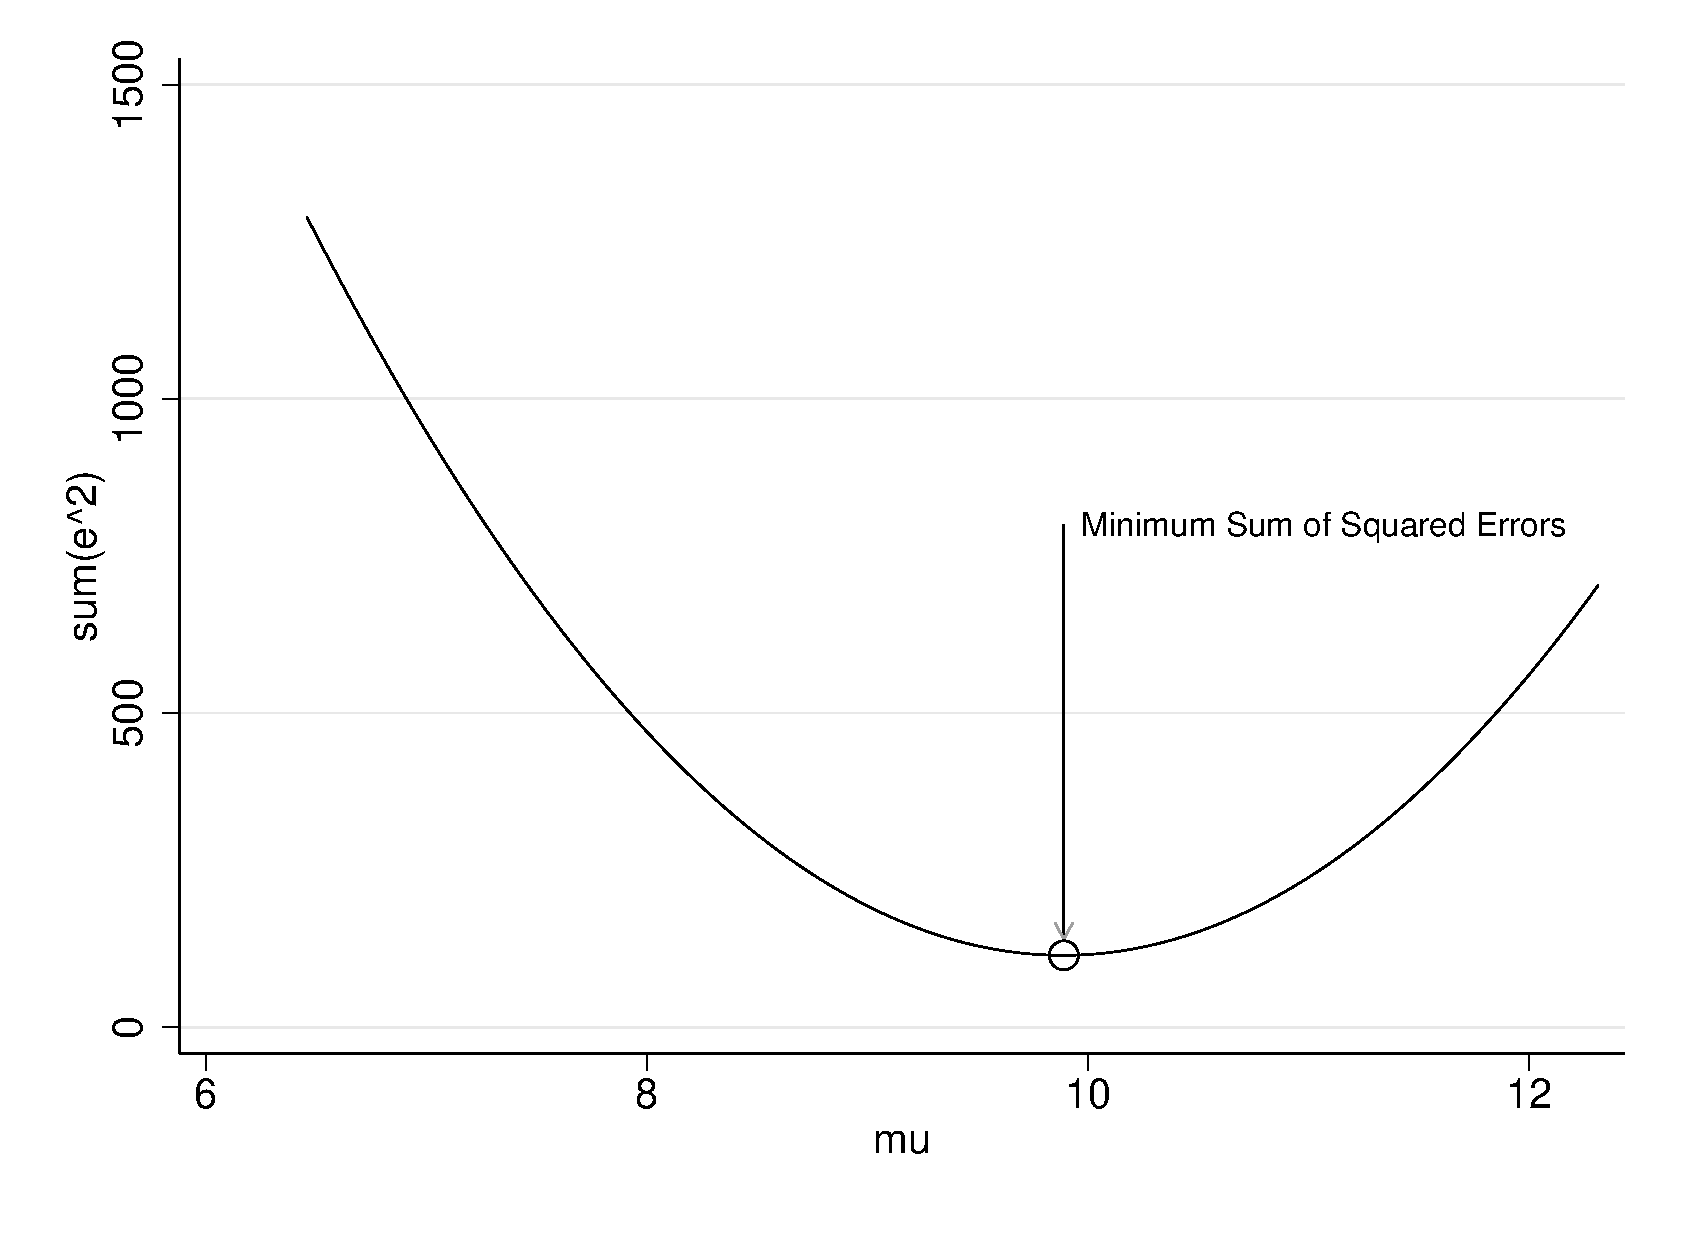
\includegraphics[angle=0,
           width=.75\textwidth]{sse.eps}
   \caption{The SSE as a function of the estimate of the mean for random variable $x$.}
  \label{fig:sse}
\end{figure}

\subsection{Maximum likelihood}
\label{sec:mimean}

Maximum likelihood is a method that expresses the probability of observing a particular parameter, given the observed data. Instead of attempting to minimize the error, this approach attempts to maximize this probability, or likelihood; hence maximum likelihood.

Each time we use maximum likelihood, we much work our parameter estimator assuming a particular distribution. Thus, if our variable is normally distributed we will use a different formula than the one for a binomial variable.

If we are dealing with a normally distributed variable, we can start with the probably of observing the $i^{th}$ value
\begin{equation}
\mbox{Pr}\left(x_i\right)=\frac{1}{\sigma\sqrt{2\pi}}\exp\left[-\frac{1}{2}\sigma^2\left(x_i-\mu\right)^2\right],
\end{equation}
and then the probability of observing a set of $x$s is then
\begin{equation}
\mbox{Pr}\left(x_i\ldots x_N\right)=\prod_{i=1}^N\frac{1}{\sigma\sqrt{2\pi}}\exp\left[-\frac{1}{2}\sigma^2\left(x_i-\mu\right)^2\right],
\end{equation}
or
\begin{equation}
\mbox{Pr}\left(x_i\ldots x_N\right)=\left(\frac{1}{\sigma\sqrt{2\pi}}\right)^N\exp\left[-\frac{1}{2}\sigma^2\sum_{i=1}^N\left(x_i-\mu\right)^2\right],
\end{equation}
we can make the formula easier if we assume that $\sigma= 1$. If we consider the probability of several {\it independent} observations, this likelihood formula becomes a function of the mean
\begin{equation}
\mbox{Pr}\left(\mu\vert x_1\ldots x_N\right)=L\left(\left(\mu\vert x_1\ldots x_N\right)\right)=\left(\frac{1}{\sqrt{2\pi}}\right)^N\exp\left[-\frac{1}{2}\sum_{i=1}^N\left(x_i-\mu\right)^2\right]
\end{equation}
We can take the log of this function to make it more tractable
\begin{equation}
\mbox{ln}\left(L\left(\mu\vert x_1\ldots x_N\right)\right)=-\frac{1}{2}\sum_{i=1}^N\left(x_i-\mu\right)^2-\frac{N}{2}\left(\mbox{ln}\left(\sqrt{2\pi}\right)\right)
\end{equation}
which is something we can handle with basic calculus. We just need to find the derivative of this function with respect to $\mu$. In this situation $\frac{N}{2}\left(\mbox{ln}\left(\sqrt{2\pi}\right)\right)$ is a constant that does not involve $\mu$, and the power rule brings the square (the 2) down as a multiplayer, and $\frac{1}{2}\times 2 = 1$, so the derivative is
\[
\frac{d\mbox{ln}\left(L\left(\mu\vert x_1\ldots x_N\right)\right)}{d\mu}=\sum_{i=1}^N\left(x_i-\mu\right)
\]
take out the sums
\[
\frac{d\mbox{ln}\left(L\left(\mu\vert x_1\ldots x_N\right)\right)}{d\mu}=\sum_{i=1}^Nx_i-N\mu
\]
set to 0 and solve
\[
0=\sum_{i=1}^Nx_i-N\mu
\]
\[
N\mu=\sum_{i=1}^Nx_i
\]
\[
\mu=\frac{\sum_{i=1}^Nx_i}{N}
\]
and there we are, the mean formula again.

\section{The proportion via maximum likelihood}
\label{sec:pml}
While the least squares principle works well for dichotomous variables (the math doesn't care if the numbers only vary between zero and one), the next step is to introduce the idea of likelihood for non-normal distributions. This will be important once we start estimating logits and probits and other models with non-normal distributions. In this section, we figure out the maximum likelihood estimate of a proportion.

Let's start with an example. A researcher takes random poll of 100 people and asks them if they like sardines. Some people said they liked sardines and were coded as 1, while others didn't like sardines and were coded as 0. The frequency table is in Table~\ref{tab:freq_x}.
\begin{table}[htbp]\centering
\caption{Frequency of dichotomous variable $y$\label{tab:freq_x}
\textbf{}}
\begin{tabular} {@{} l r r @{}} \\ \hline
Item& Number & Percent \\
\hline
0=No&    73&    73\\
1=Yes&    27&    27\\
\hline
Total&   100&   100\\
\hline
\multicolumn{3}{@{}l}{\footnotesize{\emph{$\bar{y} = 0.27$}}}
\end{tabular}
\end{table}
The researcher would like to use this data to determine the probability that someone in the population will like sardines, $y$. Of course, we would estimate the mean of this variable to get the proportion.
Why is this the right thing to do? Let's start with the function that determines the chance of observing a "1" or "0" for some variable x, given a probability p
\begin{equation}
f\left(p\vert y\right)=\mbox{Pr}\left(y=q\right)=p^q\left(1-p\right)^{1-q}, q=0,1
\end{equation}
The next important topic is the idea of a likelihood function. Researchers typically want to know the chance of observing the data they have if they assume some pre-specified model. In other words, if our model says that the chance of observing a 1 for any case is 50 percent, then how likely is it that we observed only 27 out of a 100? The likelihood function serves this purpose. It quantifies how likely we are to observe our data if we assume a specific model. In this case, our "model" is just some proportion we expect. Later, our models will become much more complicated multivariate functions. The likelihood function is
\begin{equation}
L\left(p \vert y_1 \ldots y_N\right)=\prod_{i=1}^Nf\left(y_i|p\right)
\end{equation}
To calculate the likelihood function, take the assumed chance of observing (which is $p$ for $y = 1$ and $(1 - p)$ for $y = 0$) for each case and multiply them together. (The symbol $\Pi$ works like the summation symbol, $\Sigma$, except it means multiply everything instead of adding everything). The likelihood function reduces to
\begin{equation}\label{eq:plikelihood}
L\left(p \vert y_1 \ldots y_N\right)=p^{\sum_{i=1}^Ny_i}\left(1-p\right)^{N-\sum_{i=1}^Ny_i}
\end{equation}
Which also looks scarier than it is. It's just the assumed model's probability, $p$, to the power of the total number of observed 1s times $1 - p$ to the power of the total number of observed 0s. Taking the natural log of this function gives us
\begin{equation}
\mbox{ln}\left(L\left(p \vert y_1 \ldots y_N\right)\right)=\left(\sum_{i=1}^Ny_i\right)\mbox{ln}\left(p\right)+\left(N-\sum_{i=1}^Ny_i\right)\mbox{ln}\left(1-p\right)
\end{equation}
Remember from our data that there are 27 yes answers and 100 - 27 = 73 no answers, so thus function is
\[
\mbox{ln}\left(L\left(p \vert y_1 \ldots y_N\right)\right)=\left(27\right)\mbox{ln}\left(p\right)+\left(73\right)\mbox{ln}\left(1-p\right)
\]
\begin{figure}
   \centering
   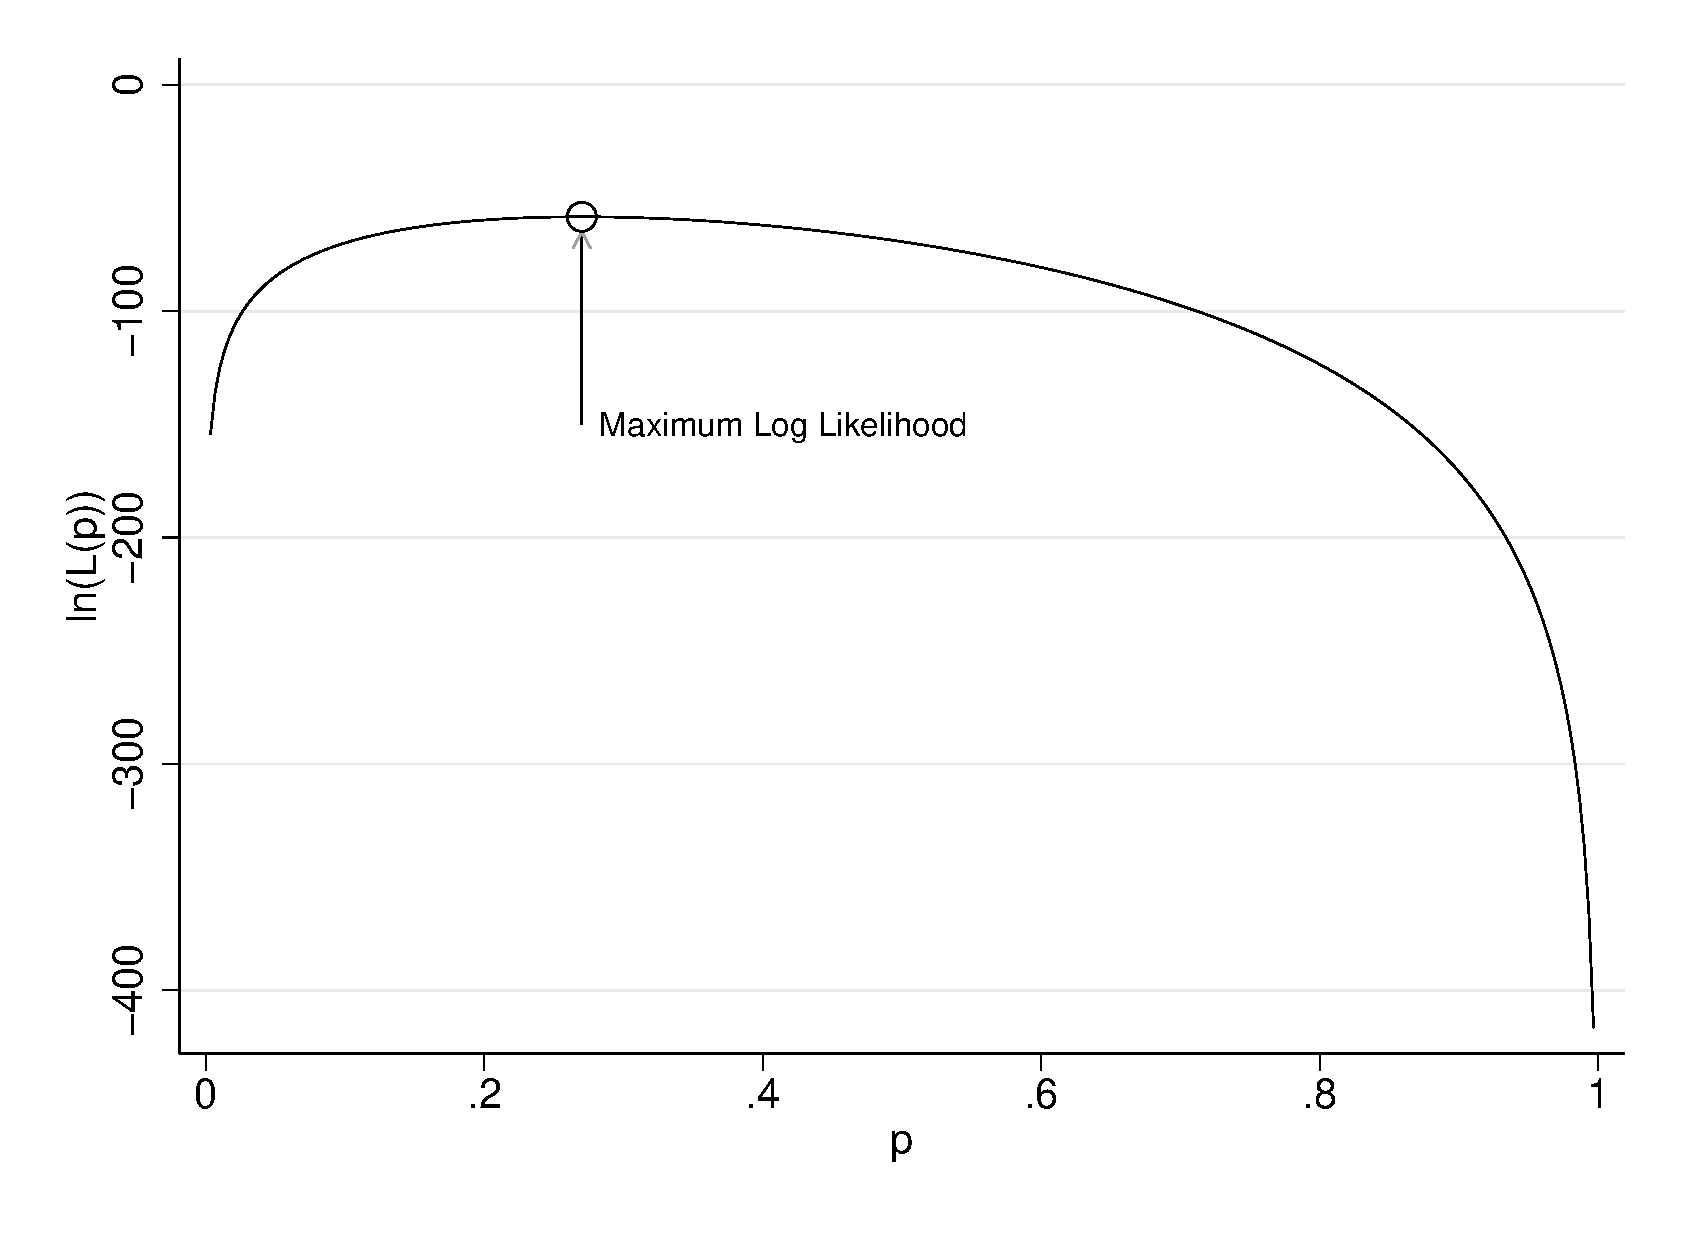
\includegraphics[angle=0,
           width=.75\textwidth]{ll.eps}
   \caption{The likelihood function for random variable $y$ with mean 0.27.}
  \label{fig:ll}
\end{figure}
Figure~\ref{fig:ll} tells a simple story: if one assumes a model where the chance of observing a 1 is the estimated mean, then the likelihood function is maximized. If any other model is assumed, the likelihood function decreases. This suggests that the optimum "model" for our data is the estimated mean. This may seem like we are going in circles, but when we have more complicated models, the idea of maximizing the likelihood of observing the data we have becomes powerful.

What process can be used to find the estimate that maximizes the likelihood? Again, the first step is to find the first derivative (which gives us an equation for slope) of this function with respect to p:
\begin{equation}
\frac{d\mbox{ln}\left(L\left(p \vert y_1 \ldots y_N\right)\right)}{dp}=\frac{\sum_{i=1}^Ny_i}{p}-\frac{N-\sum_{i=1}^Ny_i}{1-p}
\end{equation}
The next step is to set the derivative of this function to 0 (remember, when the slope is 0, the function is either at a local minima or maxima) and solve for p
\[
0=\frac{\sum_{i=1}^Ny_i}{p}-\frac{N-\sum_{i=1}^Ny_i}{1-p}
\]
\[
0=\left(\sum_{i=1}^Ny_i\right)\left(1-p\right)-\left(N-\sum_{i=1}^Ny_i\right)p
\]
\[
-\sum_{i=1}^Ny_i=-pN
\]
\[
-\frac{\sum_{i=1}^Ny_i}{N}=-p
\]
\begin{equation}\label{eq:proportion}
\frac{\sum_{i=1}^Ny_i}{N}=p
\end{equation}

\section*{For more information}
For comprehensive treatment of least squares and maximum likelihood methods, see \citep{eliason1993maximum}. For discussion of likelihood-based inference in regression models, consult \citep{fox} and \citep{gill2006essential}. Additional perspectives on numerical optimization and parameter estimation can be found in \citep{cameron2005microeconometrics}.
There we are, the formula that maximizes the likelihood is the mean, or proportion of 1s. In this case $p = 0.27$. It would be a simple matter to plug in the numbers (if they had been provided) to verify that $p = 0.27$. 